\section{Auswertung}
\label{sec:Auswertung}
\subsection{Messgrößen und Fehler}
Die Reservoire werden jeweils mit 4 Liter Wasser befüllt. Die Messdaten werden in Tabelle \ref{tab:Daten} aufgelistet. Die Wärmekapazität der Reservoire beträgt
\begin{equation}
  C_{\text{Reservoire}} = \num{750 +- 10} \frac{\text{J}}{\text{K}} \ .
  \label{eqn:c_re}
\end{equation}

\begin{table}
  \centering
  \begin{tabular}{c c c c c c}
    \toprule
    $t$ / min & $T_\text{1}$ / K & $p_\text{b}$ / kPa & $T_\text{2}$ / K & $P_\text{a}$ / kPa & Leistung / W \\
    \midrule
    0 	& 294.1 & 466	& 294.3	& 496	& 0	    \\
    1 	& 294.7 & 608	& 294.3	& 425	& 118	\\
    2 	& 295.9 & 618	& 293.2	& 446	& 120	  \\
    3 	& 296.9 & 638	& 292.5	& 466	& 125	\\
    4	& 298.2	& 628	& 291.3	& 466	& 125	\\
    5	& 299.4 & 709	& 290.2	& 466	& 125	\\
    6	& 300.7 & 730	& 289.3	& 466	& 125	\\
    7	& 302.0 & 760	& 288.5	& 455	& 125	\\
    8	& 303.2	& 790	& 287.7	& 445	& 125	\\
    9	& 304.4 & 812	& 287.0	& 425	& 124	\\
    10	& 305.5 & 820	& 286.3	& 425	& 124	\\
    11 	& 306.6 & 840	& 285.6	& 415	& 123	\\
    12	& 307.6	& 861	& 284.9	& 405	& 123	\\
    13	& 308.7 & 891	& 284.1	& 405	& 123	\\
    14 	& 309.7 & 911	& 283.5	& 395	& 123	\\
    15 	& 310.7 & 922	& 282.8	& 395	& 124	\\
    16 	& 311.6	& 963	& 282.2	& 385	& 125	\\
    17	& 312.5	& 993	& 281.5	& 385	& 125	\\
    18	& 313.5	& 1003	& 281.0	& 375	& 125	\\
    19	& 314.3	& 1023	& 280.5	& 365	& 125	\\
    20	& 315.2	& 1044	& 280.0	& 365	& 125	\\
    21	& 316.0	& 1064	& 279.5	& 365	& 125	\\
    22	& 316.8	& 1094	& 279.0	& 365	& 125	\\
    23	& 317.5	& 1104	& 278.6	& 355	& 125	\\
    24	& 318.3	& 1115	& 278.3	& 355	& 125	\\
    25	& 319.0	& 1135	& 277.9	& 355	& 125	\\
    26	& 319.8	& 1155	& 277.5	& 345	& 125	\\
    27	& 320.5	& 1175	& 277.2	& 345	& 125	\\
    28	& 321.2	& 1196	& 276.9	& 345	& 125	\\
    29	& 321.8	& 1216	& 276.6	& 345	& 125	\\
    30	& 322.5	& 1226	& 276.3	& 345	& 125	\\
    31	& 323.3	& 1236	& 276.1	& 354	& 125	\\
  \end{tabular}
  \caption{Dem Versuchsaufbau entommene Messgrößen}
  \label{tab:Daten}
\end{table}

Zu beachten ist, dass alle Messgrößen eine Messunsicherheit besitzen, einerseits einen Ablesefehler bei analogen Messinstrumenten als auch einen technischen.
\begin{eqnarray*}
  \Delta p =& &\pm 10 \cdot 10^{3} \text{p}				\\
  \Delta C =& &\pm 10 \frac{\text{J}}{\text{K}}		\\
  \Delta V =& &\pm 1.6 \cdot 10^{-3} \text{l}				\\
  \Delta \rho_{Wasser} =& &\pm 13 \frac{\text{kg}}{\text{m$^3$}}	\\
\end{eqnarray*}
Die Messunsicherheit der Dichte für Wasser kommt dadurch zu stande, dass Wasser bei verschiedenen Temperaturen seine Dichte ändert.
\subsection{Näherungsfunktion}
Mit einer nicht-linearen Ausgleichsgeraden soll der Temperaturverlauf mit Hilfe der Gleichung \ref{eqn:ausgleichsgrade} approximiert werden.
\begin{equation}
  T(t) = At^2 + Bt +C
  \label{eqn:ausgleichsgrade}
\end{equation}
Die Ermittlung der Ausgleichsgeraden erfolgt mit Hilfe von Python 3.4.3.
\begin{figure}
  \centering
  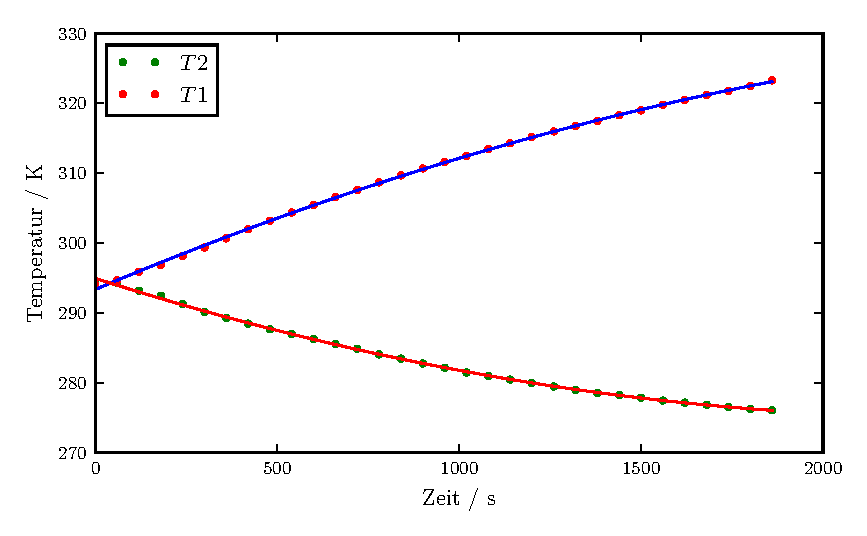
\includegraphics[width=\textwidth]{Ausgleichsgrade.pdf}
  \caption{nicht-lineare Ausgleichsgrade}
  \label{fig:ausg}
\end{figure}
Mittels einer fit Funktion werden die Koeffizienten bestimmt. Für die Temperatur $T_\text{1}$ ergeben sich die Koeffizienten
\begin{eqnarray*}
  A_1 =& (\num{-3.23 +- 0.12}) \cdot 10^{-6} \, \frac{\text{K}}{\text{s}^2}	\\
  B_1 =& (\num{2.20 +- 0.02}) \cdot 10^{-2} \, \frac{\text{K}}{\text{s}} 	\\
C_1 =& (\num{293.39 +- 0.09})  \cdot \, \text{K}
  \label{eqn:koefT1}
\end{eqnarray*}
und für $T_\text{2}$
\begin{eqnarray*}
  A_2 =& (\num{3.49 +- 0.11}) \cdot 10^{-6} \, \frac{\text{K}}{\text{s}^2} 	\\
  B_2 =& (\num{-1.67 +- 0.02}) \cdot 10^{-2} \, \frac{\text{K}}{\text{s}} 	\\
  C_2 =& (\num{294.97 +- 0.09}) \cdot \, \text{K}
  \label{eqn:koefT2}
\end{eqnarray*}
Dabei wird vernachlässigt, dass die Koeffizienten fehlerbehaftet sind, weil dies nicht mittels fit Funktion ermittelt werden kann.
\subsection{Differentialquotient}
Der Differentialquotient berechnet sich aus einmaligem Ableiten der Gleichung \ref{eqn:ausgleichsgrade} nach der Zeit.
\begin{equation}
  \frac{dT_\text{i}}{dt} = 2At + B
  \label{eqn:diffq}
\end{equation}
Aus der Funktion wird der Differentialquotient für $T_\text{1}$ und $T_\text{2}$ für vier verschiedene Zeiten berechnet. Die Ergebnisse sind in Tabelle \ref{tab:diffQ} aufgeführt.
\begin{table}
  \centering
  \begin{tabular}{c c c c c}
  	\toprule
	t / s & $T_\text{1}$ / K & $\frac{dT1}{dt}$ / $10^{-2}$ s/K & $T_\text{2}$ / K & $\frac{dT2}{dt}$ / $10^{-2}$ s/K \\
	\midrule
	60	& 294.7   & \num{2.16 +- 0.02} & 294.0 & \num{-1.62 +- 0.02} \\
	420	& 302.0   & \num{1.94 +- 0.03} & 288.5 & \num{-1.37 +- 0.02} \\
	1020	& 312.5   & \num{1.55 +- 0.03} & 281.5 & \num{-0.95 +- 0.03} \\
	1500	& 319.0   & \num{1.23 +- 0.04} & 277.9 & \num{-0.620 +- 0.004} \\
	\bottomrule
  \end{tabular}
  \caption{Differentialquotient für $T_\text{1}$ und $T_\text{2}$}
  \label{tab:diffQ}
\end{table}

\subsection{Güteziffer}
Mit Hilfe des Differentialquotienten und der Wärmekapazität der mit Wasser befüllten Reservoire
\begin{equation}
  c_\text{w} m_\text{w} = 4186.8 \cdot (\num{4 +- 0.0016}) \, \frac{\text{J}}{\text{K}} = (\num{24.9 +- 0.0}) \cdot 10^3 \, \frac{\text{J}}{\text{K}}
  \label{eqn:WC}
\end{equation}
soll die Güteziffer der Wärmepumpe bestimmt werden. Die theoretische Güteziffer lässt sich mit Hilfe der Gleichung \ref{eqn:nureal} berechnen und ist in Tabelle \ref{tab:gueteziffer} aufgeführt. Die praktisch bestimmte Güteziffer errechnet sich nach Gleichung \ref{eqn:nureal} aus der Wärmekapazität der Reservoire und der Wärmekapazität der Leitungen sowie mit den in Tabelle 1 bestimmten Differentialquotienten, sowie mit der nach Formel \ref{eqn:ave} und \ref{eqn:var} gemittelten Leistung.
\begin{table}
  \centering
  \begin{tabular}{c c c}
    \toprule
    $t$ / s & $\nu_\text{theo}$ & $\nu_\text{exp}$ \\
    \midrule
    60	 & \num{700 +-100} 	& \num{3.04 +- 0.05} 	\\
    420  & \num{22.4 +- 0.1}	& \num{2.72 +- 0.05} 	\\
    1020 & \num{3.2 +- 0.6}	& \num{2.17 +- 0.05}	\\
    1500 & \num{2.8 +- 0.5}	& \num{1.73 +- 0.06} 	\\
    \bottomrule
  \end{tabular}
  \caption{theoretisch und praktisch bestimmte Güteziffer}
  \label{tab:gueteziffer}
\end{table}
Gründe für die Abweichung zwischen der theoretischen Güteziffer und der experimentell ermittelten Güteziffer werden in der Diskussion aufgeführt.
\subsection{Dampfdruckkurve}
Die Verdampfungswärme $L$ wird mit Hilfe einer Verdampfungskurve ermittelt. In Tabelle \ref{tab:Dampfdruck} sind die Dürcke mit den entsprechenden Temperaturen aufgelistet.
\begin{table}
  \centering
  \begin{tabular}{c c}
    \toprule
	$p$ / bar & $T$ / Kelvin\\
    \midrule
    	0	& -60	\\
	1	& -30	\\
	2	& -12	\\
	3	& -1	\\
	4	&  8	\\
	5	&  15	\\
	6	&  23	\\
	7	&  28	\\
	8	&  33	\\
	9	&  39	\\
	10	&  42	\\
    \bottomrule
  \end{tabular}
  \caption{Wertepaare zur Dampfdruckkurve von $Cl_2F_2C$}
  \label{tab:Dampfdruck}
\end{table}
Dafür wird im Diagramm \ref{fig:dampfdruck}
\begin{figure}
  \centering
  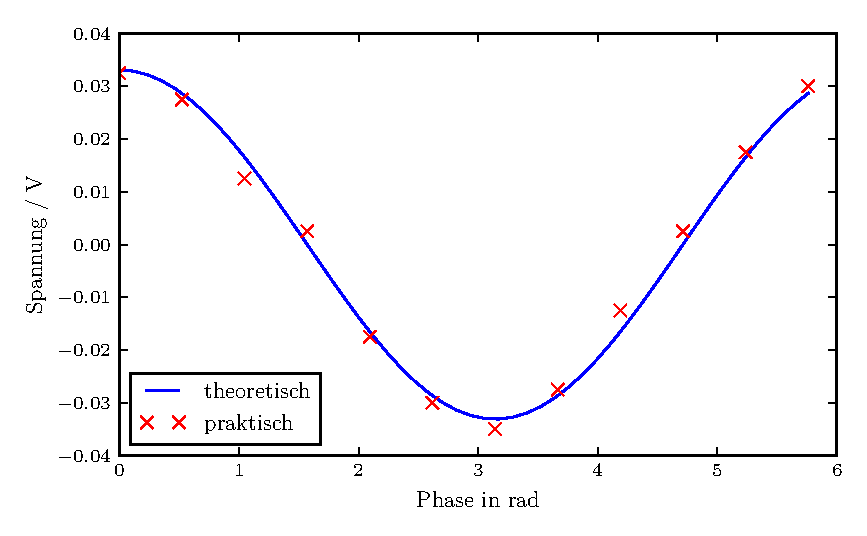
\includegraphics[width=\textwidth]{Dampfdruck.pdf}
  \caption{Dampfdruckkurve}
  \label{fig:dampfdruck}
\end{figure}
$1/T$ gegen $log(p/p_0)$ aufgetragen und die Steigung der Graden in die Formel \ref{eqn:dampfgl} eingesetzt.
\begin{equation}
  L = log \left( \frac{p}{p_o} \right) \cdot T \cdot \frac{1}{R}
  \label{eqn:dampfgl}
\end{equation}
Die Steigung der Ausgleichsgeraden wird mittels einer linearen Regression berechnet und beträgt
\begin{equation*}
  m = \num{-2430 +- 20} \, \text{s} \ .
\end{equation*}
Daraus ergibt sich eine Verdampfungswärme von
\begin{equation}
  L = (\num{20200 +- 170}) \, \frac{\text{J}}{\text{K}} \ .
\end{equation}
\subsection{Massendurchsatz}
Die Verdampfungswärme wird nun in Formel \ref{eqn:dm/dt} eingesetzt und damit der Massendurchsatz ermittelt. Die Massendurchsätze der verschiedenen Zeiten sind in Tabelle \ref{tab:dm/dt} aufgetragen. Sie werden mit der Molaren Masse von Dicholdifluormethan multipliziert um sie für die weiteren Aufgabenteile bereits umzurechen. 
\begin{equation}
  M_{\text{Dichlordifluormethan}} = 120.91 \frac{g}{mol} \ \text{\cite{M}}
\end{equation}
\begin{table}
  \centering
  \begin{tabular}{c c c}
    \toprule
    $T$ / s & $\frac{dm}{dt}$ / (mol/s) & $\frac{dm}{dt}$ / (g/s) \\
    \midrule
    60   & \num{0.0140 +- 0.0002} & \num{1.69 +- 0.02}\\
    420  & \num{0.0119 +- 0.0002} & \num{1.44 +- 0.02}\\
    1020 & \num{0.0082 +- 0.0003} & \num{1.00 +- 0.04}\\
    1500 & \num{0.0053 +- 0.0003} & \num{0.64 +- 0.04}\\
    \bottomrule
  \end{tabular}
  \caption{Massendurchsatz $dm/dt$}
  \label{tab:dm/dt}
\end{table}
Für die weiteren Rechnungen wird der Massendurchsatz durch Multiplikation mit der Molaren Masse in die SI-Einheit umgerechnet.
\subsection{Mechanische Kompressorleistung}
Aus der idealen Gasgleichung lässt sich die Dichte in den Rohren berechnen. Dafür muss jedoch die Dichte von Dichlordifluormethan bei 1 Bar Druck und 273 Kelvin bekannt sein.
\begin{equation}
  \rho_\text{0} =  5.51 \, \frac{\text{g}}{\text{l}} \ \text{\cite{rho}} \ .
  \label{rho}
\end{equation}
Zusätzlich wird gefordert, dass
\begin{equation}
  nR = konstant
\end{equation}
ist und das die Dichte homogen verteilt ist. Daraus lässt sich die ideale Gasgleichung umstellen und man erhält
\begin{eqnarray*}
  \frac{pV}{T} =nR =& konstant \\
  \frac{p_0 V_0}{T_0} = \frac{p_2 V_2}{T_\text{2}}  \Leftrightarrow&  \frac{p_0 m}{\rho_0 T_0} = \frac{p_2 m}{T_\text{2} \rho_2} \\
  \frac{p_0}{\rho_0 T_0} = \frac{p_2}{T_\text{2} \rho} \Leftrightarrow& \rho = \frac{\rho_o T_o P_2}{T_\text{2} P_0}
  \label{eqn:rho}
\end{eqnarray*}
einen Ausdruck für die Dichte in Abhängigkeit der Temperaturen und Drücke. Dies wird in Formel \ref{eqn:nmech} eingesetzt und die Ergebnisse für die verschiedenen Zeitpunkte in Tabelle \ref{tab:LdK} eingetragen.
\begin{table}
  \centering
  \begin{tabular}{c c c}
    \toprule
    $t /$ s & $\rho /$ $\frac{10^{-3}kg}{l}$ & N / W \\
    \midrule
    60   & \num{21.7 +- 0.5} & \num{10.6 +- 0.7} \\
    420  & \num{23.7 +- 0.5} & \num{12.8 +- 0.5} \\
    1020 & \num{20.6 +- 0.5} & \num{16.4 +- 0.6} \\
    1500 & \num{19.2 +- 0.5} & \num{13.0 +- 0.9} \\
    \bottomrule
  \end{tabular}
  \caption{Leistung des Kompressors}
  \label{tab:LdK}
\end{table}
